\documentclass{article}
% For Images and tables formatting 
\usepackage{graphicx} % Required for inserting images
\usepackage{booktabs} % Required for tables
\usepackage{float} % For floating configurations
\usepackage{multirow} % For combining rows in a table
\usepackage{ragged2e} % For justifying setting
\usepackage{titlesec} % For headers formatting

% For Page settings
\usepackage{tabularx} % For automated columns sizing 
\usepackage{geometry} % For margin settings

% For paragraph settings
\setlength{\parskip}{1em}   % Adds vertical space between paragraphs
\setlength{\parindent}{0pt} % Removes indentation

% For bibliography and references
\usepackage[backend=biber, style=apa]{biblatex} % APA style, uses Biber
\addbibresource{References.bib} % Specify .bib file
\usepackage{csquotes} % For advanced quotations handlings

% For math 
\usepackage{amsmath,amssymb,amsfonts} % For math fonts, symbols and environments

%For specific sections of the document
\usepackage{abstract}

\title{\textbf{Desarrollo de una membrana cerámica a partir de Pumicita y Ceniza de Bagazo de Caña de Azúcar (CBCA) mediante colaje tradicional para procesos de microfiltración.}}
\author{\textbf{Sergio A. Bustamante$^1$, Lester J. Espinoza$^2$, Rolando A. Guevara$^3$}\\ $^1$Área de Conocimiento de Agricultura, Universidad Nacional de Ingeniería, Managua, Nicaragua\\ $^2$Área de Conocimiento de Agricultura, Universidad Nacional de Ingeniería, Managua, Nicaragua\\ $^3$Área de Conocimiento de Agricultura, Universidad Nacional de Ingeniería, Managua, Nicaragua}
\date{}

\titleformat{\section}[block]{\normalfont\Large\bfseries\centering}{\thesection}{1em}{}

\begin{document}
\maketitle

\begin{center}
    \textbf{\large{ABSTRACT} }
\end{center}

\justifying
In this study, ceramic membranes were developed using Pumice (Pum) and Sugarcane Bagasse Ash (SCBA), sourced from a sugar mill in Nicaragua, as the main precursor powders. The membranes were shaped into circular disks and sintered at 800 °C for 4 hours. Two Pum/SCBA ratios and two heating rates were investigated to assess their influence on apparent porosity, density, and pore size. The resulting membranes were characterized through chemical stability tests and water permeation assays with ash suspensions. The results indicate that membranes with higher CBCA content and lower heating rates exhibit greater porosity and reduced pore diameter, consistent with partial vitrification and densification mechanisms. Chemical stability tests revealed that CBCA-rich membranes are more susceptible to acid attack due to the presence of soluble phases, while showing lower reactivity in alkaline media. Microfiltration assays demonstrated that membranes sintered at lower heating rates achieved higher pure water flux, with M4 membranes outperforming M2 due to their enhanced porosity. These findings support the viability of pumice–CBCA ceramic composites for low-cost water treatment applications, particularly in contexts requiring selective filtration and material sustainability.
\hfill \break

\textbf{key words:} Membrane separations; Ceramic forming; Paste casting; Microfiltration. 

\begin{center}
    \textbf{\large{RESUMEN} }
\end{center}

\justifying
En este estudio, se desarrollaron membranas cerámicas a partir de Pumicita (Pum) y Ceniza de Bagazo de Caña de Azúcar (CBCA), proveniente de un Ingenio en Nicaragua, como polvos precursores principales. Las membranas fueron conformadas en discos circulares y sinterizadas a 800 °C por 4 horas. Dos proporciones de Pum/CBCA y dos tasas de calentamiento fueron investigados para evaluar su influencia en la porosidad, densidad y tamaño de poros aparente. Las membranas resultantes fueron caracterizadas a través de pruebas de estabilidad química y ensayos de permeación de agua con suspensiones de ceniza. Los resultados indican que Los resultados indican que las membranas con mayor contenido de CBCA y sinterizadas a tasas de calentamiento bajas presentan una mayor porosidad y una reducción en el diámetro de poro, en concordancia con los mecanismos de vitrificación parcial y densificación. Las pruebas de estabilidad química revelaron que las membranas ricas en CBCA son más susceptibles al ataque ácido debido a la presencia de fases solubles, mientras que muestran menor reactividad en medios alcalinos. Los ensayos de microfiltración demostraron que las membranas sinterizadas a tasas bajas alcanzan mayores valores de flujo de agua pura, siendo las membranas tipo M4 superiores a las tipo M2 por su mayor porosidad. Estos hallazgos respaldan la viabilidad de los compósitos cerámicos Pumicita–CBCA como alternativa de bajo costo para aplicaciones en tratamiento de agua, especialmente en contextos que requieren filtración selectiva y sostenibilidad material.

\textbf{Palabras claves:} Separación por membrana; Conformado cerámico; Colaje tradicional de pastas; Microfiltración. 

\newpage
\section{INTRODUCCIÓN}

El acceso a tecnologías eficientes para el tratamiento de agua es un desafío persistente, especialmente en contextos donde la sostenibilidad, el uso de materiales locales y de bajo costo son factores determinantes. Entre las alternativas más prometedoras, los procesos de separación por membranas han demostrado alta eficacia para remover contaminantes presentes en aguas naturales y residuales, permitiendo la retención selectiva de partículas suspendidas, coloides, microorganismos y iones sin la generación excesiva de subproductos o lodos.

Tradicionalmente las membranas cerámicas han sido fabricadas a partir de óxidos metálicos como el óxido de titania y circonia por la producción de membranas altamente estables y eficientes pero de costos elevados (\cite{Gitis2016,Nandi2008}). Por esta razón, recientes investigaciones se han llevado a cabo con el fin de obtener membranas cerámicas utilizando materiales alternativos, no metálicos, de bajo costo y requerimiento energético, tales como el polvo de apatita (\cite{Masmoudi2007}),  la ceniza volante (\cite{Saffaj2004}), la arcilla natural (\cite{Saffaj2005}), Caolín (\cite{Rawat2018}) y Ceniza de Bagazo de Caña de Azúcar (\cite{Andrade2019}). 

Sin embargo, el desarrollo de un compósito cerámico a partir de Pumicita y Ceniza de Bagaso de Caña de Azúcar (CBCA), proveniente de un ingenio Nicaragüense, para la fabricación de membranas cerámcias no ha sido reportado previamente por la literatura. Por esta razón, el presente trabajo tiene como objetivo el desarrollo de una membrana cerámica funcional, orientada a aplicaciones de microfiltración de agua, empleando materiales locales y procesos de sinterizado accesibles. 


\newpage
\section{MATERIALES Y MÉTODOS}
\subsection{Materiales y reactivos}
Los materiales inorgánicos principales utilizados en este trabajo para la conformación de las membranas cerámicas fueron la pumicita, ceniza de bagazo de caña de azúcar (CBCA), carbonato de calcio, carbonato de sodio, ácido bórico y metasilicato de sodio, este último en solución al 35\%. 


Estos materiales fueron introducidos en la estructura de la pasta cerámica por los atributos funcionales que pueden aportar a las características de la pieza final. Utilizando el esquema de clasificación de \textcite{Benito2004} para los agregados o aditivos utilizados en la conformación de membranas cerámicas, se utilizaron como agentes ligantes el ácido bórico y silicato de sodio. Por su parte, el carbonato de calcio fue adicionado por su doble función como agente ligante y modificador estructural en términos de porosidad, y el carbonato de sodio como un defloculante y modificador de tamaños de poros en la membrana. 

Por su parte, referente a los polvos precursores principales, la CBCA ha sido desmostrado que, al ser empleada en la fabricación de membranas cerámicas, funciona como un agente formador de poros (\cite{Andrade2019}). En cuanto a la pumicita, fue utilizada por su capacidad de proporcionar la estructura y porosidad base de la pieza, debido a su alto contenido de sílice y alúmina.  

La pumicita utilizada fue obtenida de un vivero local, mientras que la CBCA fue proporcionada por el Ingenio Monte Rosa del Grupo Pantaleón. Por su parte, los demás reactivos fueron proporcionados por la Universidad Nacional de Ingeniería, Managua. 

El tamizado, tanto de la pumicita y la ceniza como de los demás reactivos, fue realizado utilizando tamices estándar de aluminio de 8 in cuyos arreglos se muestran en la Figura 1. Para el tamizado de los polvos principales (pumicita y ceniza) y reactivos se utilizó un arreglo de tamices No. 8, 35, 50, 80, 140 y 230. 

\subsection{Preparación de las membranas}

Se prepararon 5 tipos de membranas como se muestran en la tabla \ref{tab:Composicion Membranas}. 

\begin{table}[ht]
\caption{Composición de las membranas desarrolladas}
    \centering
    \begin{tabular}{p{3cm} p{2cm} p{2cm} p{2cm} p{2cm} p{2cm}}
         \toprule
        \multirow{2}{*}{Materia Prima} & \multicolumn{5}{c}{Cantidad usada (\% en peso)} \\
        \cline {2-6} 
        & M1 & M2 & M3 & M4 & M5 \\  
         \midrule
        Pumicita & 75 & 50 & 37,5 & 25 & 0 \\
        CBCA     &  0 & 25 & 37,5 & 50 & 75 \\
        $CaC\mathrm{O}_3$ & 15 & 15 & 15 & 15 & 15 \\
        $N\mathrm{a}_2C\mathrm{O}_3$ & 5 & 5 & 5 & 5 & 5 \\
        Acido borico     &  2,5 & 2,5 & 2,5 & 2,5 & 2,5 \\
        $N\mathrm{a}_2Si\mathrm{O}_3$ & 2,5 & 2,5 & 2,5 & 2,5 & 2,5 \\
         \bottomrule
    \end{tabular}
    \label{tab:Composicion Membranas}
\end{table}

Los polvos principales y reactivos fueron mezclados con suficiente agua destilada para obtener una pasta o suspensión cerámica, la cual fue introducida en un moldeador diseñado específicamente para el conformado de las pastas cerámicas mostrado en la figura \ref{fig:Moldeador_Pastas}. De esta manera se obtuvieron piezas en verde de forma circular con diámetro de 52-59 mm y espesor de 8-12 mm . 

\begin{figure}[ht]
    \centering
    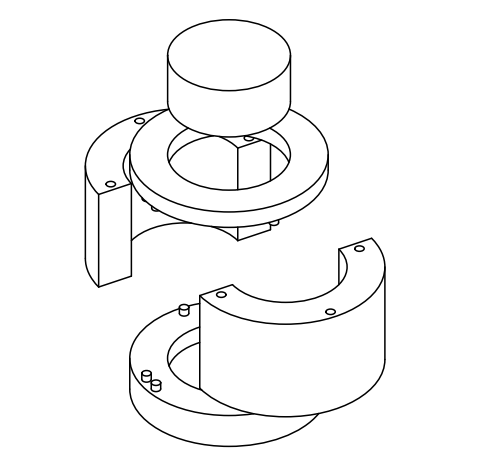
\includegraphics[width=0.4\linewidth]{Graphics/Moldeador ZTMY-01.png}
    \caption{Moldeador de pastas}
    \label{fig:Moldeador_Pastas}
\end{figure}

Para la primera parte del secado al ambiente, la pasta cerámica fue mantenida por 24 horas dentro del conformador. Al cabo de este tiempo, la pieza moldeada fue removida cuidadosamente del conformador e introducida a un desecador con sílica gel seca por un período de 24 a 72 horas, para la segunda parte del secado al ambiente. Las piezas que salen del proceso de secado al ambiente se denominaron ‘Piezas en verde’.

Posteriormente, las piezas en verde fueron introducidas a un horno convectivo marca Fisherbrand modelo Isotemp Serie 500, precalentado a 40°C hasta 60°C por un tiempo de 24 horas hasta que la pieza experimentó un cambio de color de gris oscuro a gris claro, lo cual representa una disminución del porcentaje de humedad de la pieza en verde del 60\% - 70\% en base a las observaciones realizadas experimentalmente. 

Luego, las piezas resultantes del secado en horno, sin macro fracturas, fueron introducidas a una mufla marca Thermo Scientific Thermolyne modelo FB1310M a 800 °C con tiempos (4 y 8 horas) y tasas de calentamiento variables (4.75 °C/min y 6.82 °C/min). Las membranas obtenidas del proceso de sinterizado fueron denominadas ‘Membranas precursoras’.

Por último, las membranas precursoras fueron pulidas con un papel abrasivo de Óxido de Aluminio número 40 hasta un espesor promedio de 6 mm, para lograr una superficie uniforme y adecuada para adaptar los componentes utilizados en las pruebas de microfiltración y prevenir las fugas de fluido o presión. Las membranas pulidas fueron denominadas ‘Membranas cerámicas finales’. Un resumen del proceso se muestra en la Figura \ref{fig:Esq_PrepMembranas}.

\begin{figure}[ht]
    \centering
    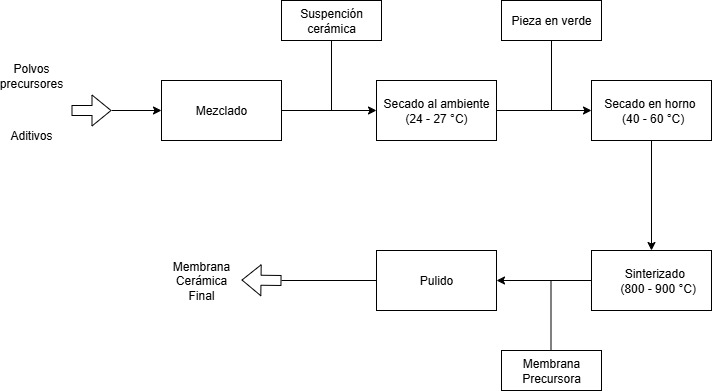
\includegraphics[width=0.7\linewidth]{Esquema de preparacion de membranas ceramicas.jpg}
    \caption{Esquema de preparación de las membranas conformadas}
    \label{fig:Esq_PrepMembranas}
\end{figure}

\subsection{Caracterización de las membranas}

Las membranas conformadas fueron sometidas a pruebas de estabilidad química, en las cuales las membranas fueron sumergidas en soluciones ácidas y alcalinas durante un período de siete dias. Para la inmersión en medio ácido, fue utilizada una solución de ácido clorhídrico (HCl) 12.1 N, pH = 1. Para la inmersión en medio alcalino, se utilizó una solución de hidróxido de sodio (NaOH) concentrado, pH = 13. 

Previo a cada inmersión, se tomaron los valores de peso y porcentaje de humedad de la membrana. Al cabo de dos días, las membranas fueron secadas en un horno a 120°C por 3 horas en promedio. Se midió porcentaje de humedad en las membranas como un criterio de calidad del secado; en caso de que la humedad fuera mayor a la inicial previa a la inmersión, la membrana era devuelta al horno para continuar con el proceso de secado, en caso contrario, se pesó la membrana en una balanza analítica. Este proceso se repitió a lo largo de los siete días de la prueba. 

El porcentaje de pérdida de peso fue calculado mediante la ecuación \ref{Eq:Perdida_Peso}. Donde P0 representa el peso, en gramos, tomado previo a la inmersión, Px representa el peso, en gramos, tomado en el día x de la inmersión y \%P(x) representa el porcentaje de pérdida de peso en función de x días de inmersión en la solución.   

\begin{equation}
    \%P(x) = \frac{P_0-P_x}{P_0} \times 100
    \label{Eq:Perdida_Peso}
\end{equation}

El cálculo de la porosidad aparente de cada membrana final obtenida utilizando la metodología descrita por \parencite[p~122]{Purkait2018}. Esta metodología consistió en sumergir la membrana en un recipiente con agua destilada por un tiempo de al menos 12 horas. Una vez transcurrido el tiempo, la membrana húmeda fue retirada del recipiente y secada con un trozo de tela de microfibra para escurrir el agua en exceso en la superficie de la membrana. Esta membrana húmeda fue pesada y luego secada en un horno a 120 °C por dos horas. Se verificó el porcentaje humedad de la membrana mediante la balanza de humedad, para asegurar que este porcentaje fuera menor o igual al porcentaje inicial obtenido al finalizar la etapa de pulido. 

El porcentaje de porosidad aparente (P.A) se obtuvo por método gravimétrico de acuerdo con la ecuación \ref{Eq:Porosity}. Donde, $W_w$ es el peso de la membrana húmeda (g), $W_d$ es el peso de la membrana seca (g), $\rho$ representa la densidad del agua ($g/m^3$) a temperatura ambiente y V el volumen de la membrana ($m^3$).

\begin{equation}
    P.A = \frac{W_w-W_d}{\rho \times V}
    \label{Eq:Porosity}
\end{equation}

Para la estimación del diámetro de poros se adaptó la ecuación \ref{Eq:DiametroPoros} utilizada para el método de punto burbuja, utilizando un sistema de microfiltración compuesto por una bomba de vacío, un kitasato, un soporte, una membrana y un embudo. De esta manera, la presión reportada corresponde a la presión a la cual el líquido mojante pasa a través de la estructura porosa, permitiendo realizar una aproximación al diámetro de poros en la membrana. 

\begin{equation}
    D_p = \frac{288}{P_{bp}}
    \label{Eq:DiametroPoros}
\end{equation}

Las pruebas de permeación fueron realizadas utilizando el arreglo que se muestra en la figura \ref{fig:Arreglo_MF}. 

\begin{figure}
    \centering
    \includegraphics[width=0.5\linewidth]{Graphics/Sistema de filtración-Layout1.png}
    \caption{Arreglo para pruebas de microfiltración}
    \label{fig:Arreglo_MF}
\end{figure}

\section{RESULTADO Y DISCUSIÓN}
\subsection{Acondicionamiento y selección de los polvos principales y reactivos}

El tamaño de partículas máximo para los polvos utilizados fue de 63 $\mu m$ debido a la limitada disponibilidad de tamices de menor tamaño. Para alcanzar la homogeneidad de tamaño de partículas en los polvos precursores y reactivos se realizaron algunas operaciones unitarias previas al tamizado, para la selección de partículas con tamaños en el rango deseado. 

Para la pumicita, debido a su gran tamaño, en comparación con las demás materias primas, fueron necesarias las operaciones de lavado, secado, molienda y tamizado para su limpieza, reducción de tamaño y selección de partículas. Por su parte, para la CBCA, carbonato de sodio y ácido bórico, solamente fue necesaria una etapa de molienda previo al tamizado para asegurar la mayor cantidad de partículas con tamaños menores a 63 $\mu m$. 

Las curvas de distribución de tamaño de partículas completa para los polvos principales y reactivos se muestran en la figura \ref{fig:Distribucion_Particulas}, sin embargo, solamente las partículas de tamaños menores a 63 $\mu m$ fueron utilizadas para la fabricación de las membranas cerámicas para asegurar una distribución de tamaños angosta, lo cual es beneficioso de acuerdo a con lo investigado por \textcite{Lin1995} para mejorar la tasa de densificación y el crecimiento de granos como lo menciona \textcite{Kang2020}. 

Por lo tanto, la fracción aprovechable es del 90.76\%, 62.63\%, 46.45\%, 82.97\% y 19.2\% para la Pumicita, CBCA, $CaCO_3$, $Na_2CO_3$ y ácido bórico respectivamente, para la conformación de las membranas cerámicas. 

\begin{figure}[ht]
    \centering
    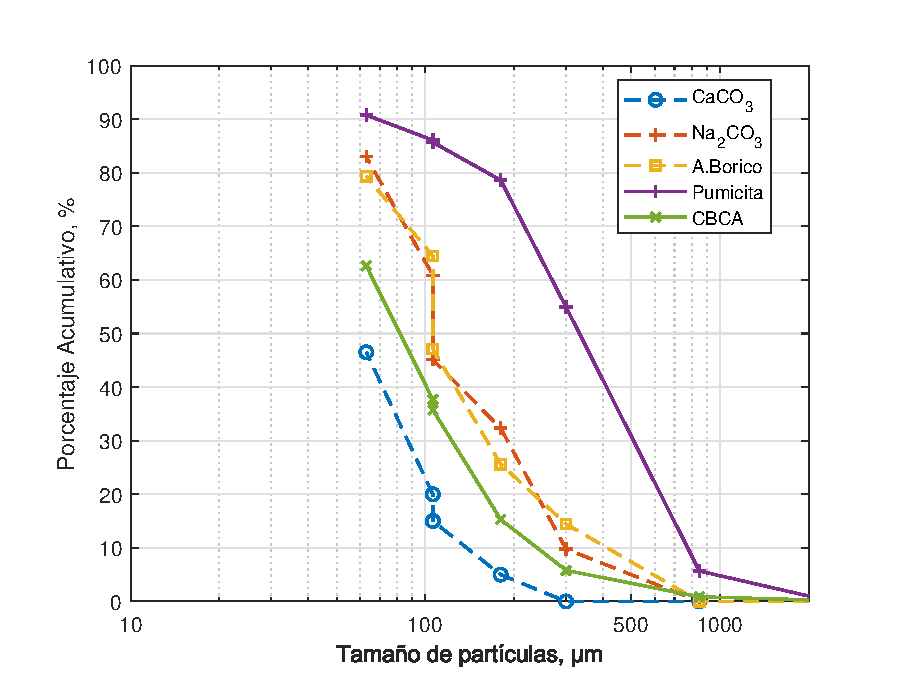
\includegraphics[width=0.7\linewidth]{Graphics/ParticleDistributionC.eps}
    \caption{Curvas de distribución de tamaño de las materias primas}
    \label{fig:Distribucion_Particulas}
\end{figure}

\subsection{Conformación de las membranas cerámicas}

En la Figura \ref{fig:Pasta_Cerámica} se muestra la suspensión cerámica obtenida tras el mezclado de los polvos y reactivos. Los resultados experimentales evidencian que un exceso de humedad, así como la falta de homogeneidad en la mezcla (manifestada por la presencia de grumos), favorece la aparición de defectos y agrietamiento en etapas tempranas del conformado.

Por esta razón, se prepararon suspensiones con diferentes contenidos de agua. Se encontró que, para todas las membranas (M1–M5) elaboradas a partir de pumicita y CBCA, un contenido de agua inferior al 76\% (en base al peso total) no permite formar una suspensión homogénea, ya que aparecen grumos por zonas sin hidratar. En cambio, contenidos superiores al 90\% representan un exceso de agua que dificulta el manejo.

El contenido óptimo de agua dependió de la fracción de CBCA: en promedio, 76\% - 80\% para membranas de tipo M1 (100\% pumicita) y 88\% - 90\% para membranas de tipo M5 (100\% CBCA). Este rango permitió obtener una pasta con comportamiento pseudoplástico, propio de un fluido no newtoniano, lo cual favorece el conformado con el moldeador mostrado en la Figura \ref{fig:Moldeador_Pastas}.

\begin{figure}[ht]
    \centering
    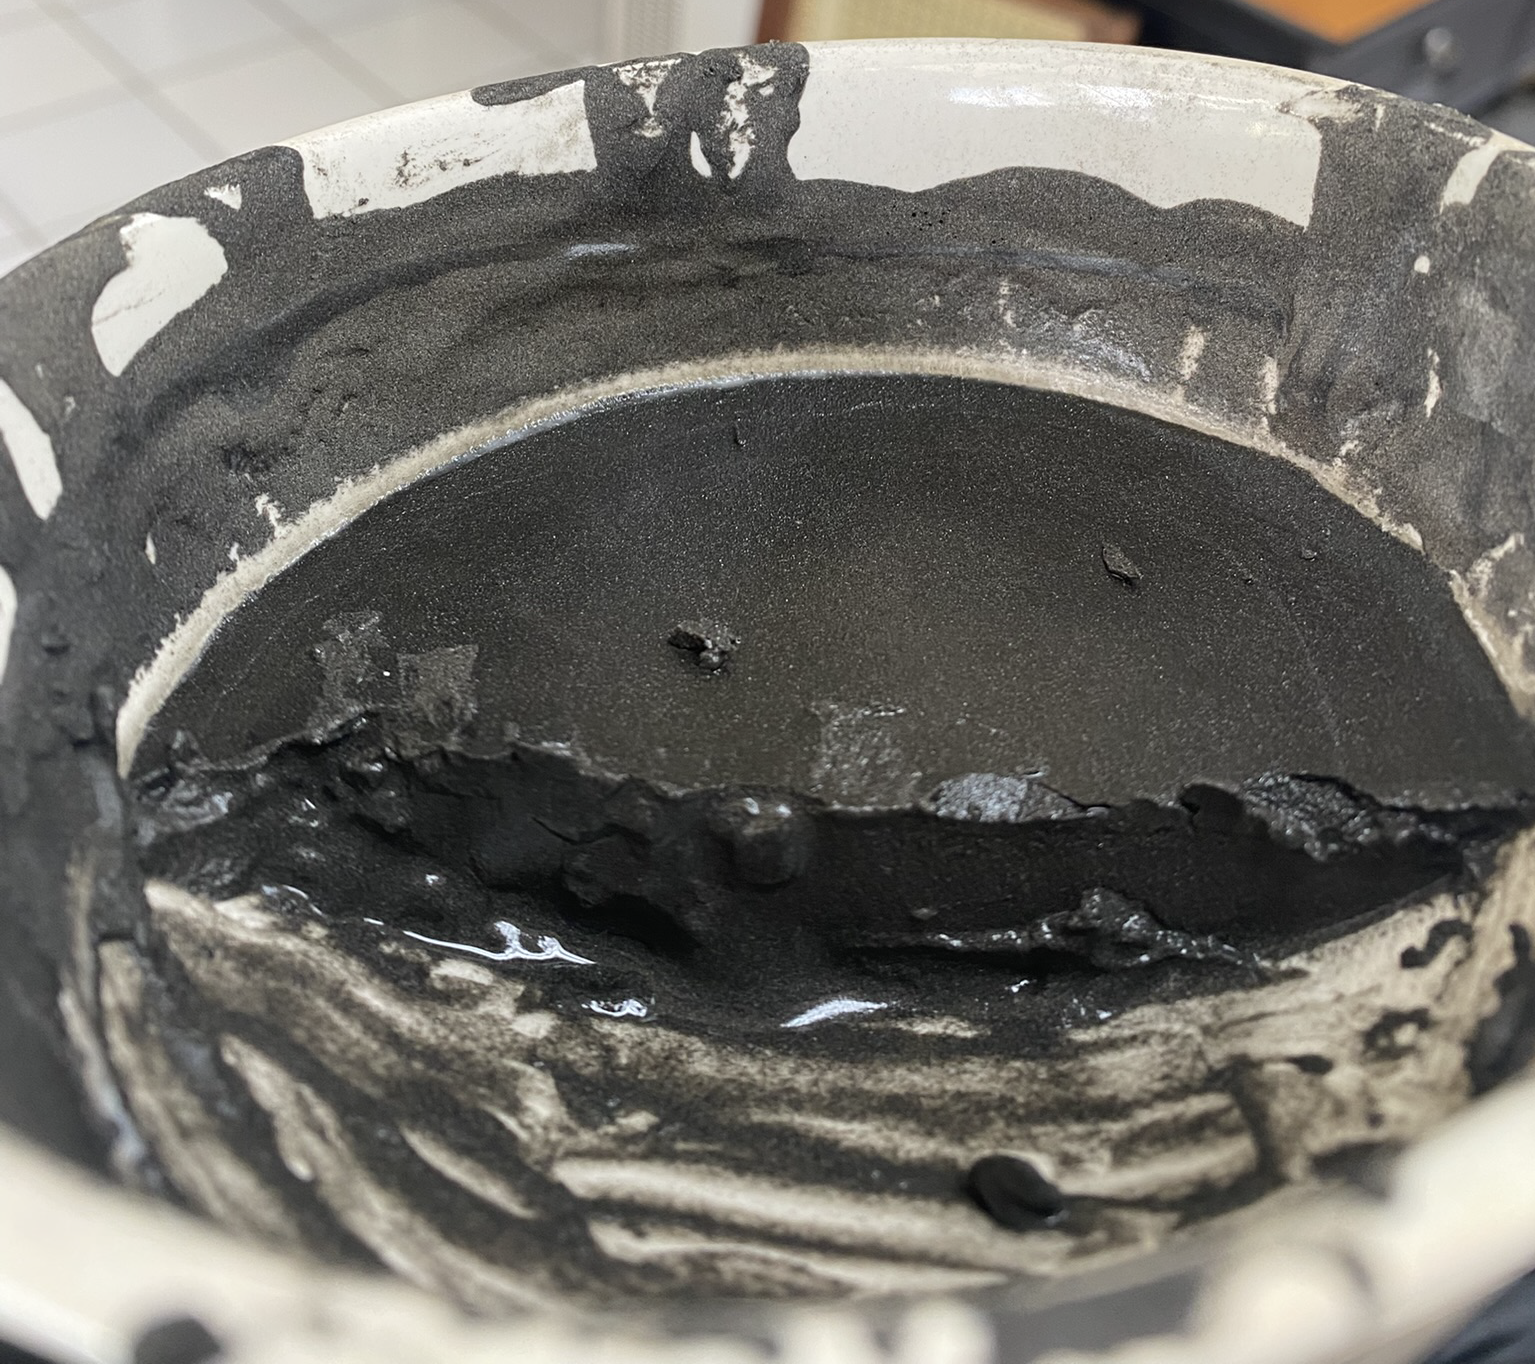
\includegraphics[width=0.5\linewidth]{Graphics/Suspension ceramica.png}
    \caption{Pasta o suspensión cerámica}
    \label{fig:Pasta_Cerámica}
\end{figure}

El secado en hornos es una de las etapas más fundamentales para la prevención de fracturas en la membrana ya que, de acuerdo con las experimentaciones realizadas, cerca del 87 \% de fracturas nuevas aparecieron en las piezas en las primeras 2 horas durante el proceso de secado en hornos por altas temperaturas de secado o cambios bruscos de temperatura. Del 13 \% restante, 10 \% de las fracturas aparecieron durante los primeros procesos de conformación y secado al ambiente por exceso o deficiencia de humedad en la pieza como se mencionó anteriormente y solamente un 3 \% aparecieron durante el proceso de sinterizado. Por lo que, al mantener una temperatura de 40 °C - 60 °C durante las primeras 3 horas y posteriormente hasta 150 °C por 5 horas, se redujeron drásticamente la cantidad de fracturas presentes en la pieza. 
 
Durante el proceso de sinterizado, la cantidad de nuevas fracturas que aparecieron en la estructura de la membrana es relativamente poca en comparación con los otros procesos previos. Sin embargo, la aparición de nuevas fracturas usualmente se debió a una tasa de calentamiento muy alta y alto porcentaje de humedad en la pieza. El tiempo de sinterizado no tuvo efectos en la aparición de nuevas fracturas en las membranas precursoras. 

No obstante uno de los efectos más notorios ocurridos durante el proceso de sinterizado para membranas de Pumicita/CBCA es la aparición del efecto de la vitrificación parcial, especialmente en los bordes de las piezas como se muestra en la figura \ref{fig:vitrification}. En esta figura se presentan dos regiones, una inferior caracterizada por una apariencia vidriosa y otra más granular/porosa en la parte superior. 

Este efecto puede atribuirse a la presencia de óxidos alcalinos y alcalinotérreos en la CBCA ($K_2O$, $Na_2O$, $CaO$, $MgO$), que actúan como fundentes al reducir la temperatura de fusión de la sílice. Como consecuencia, se forma una fase vítrea que promueve la densificación por cierre parcial de poros, lo cual modifica la porosidad y la permeabilidad final de las membranas. 

\begin{figure}[ht]
    \centering
    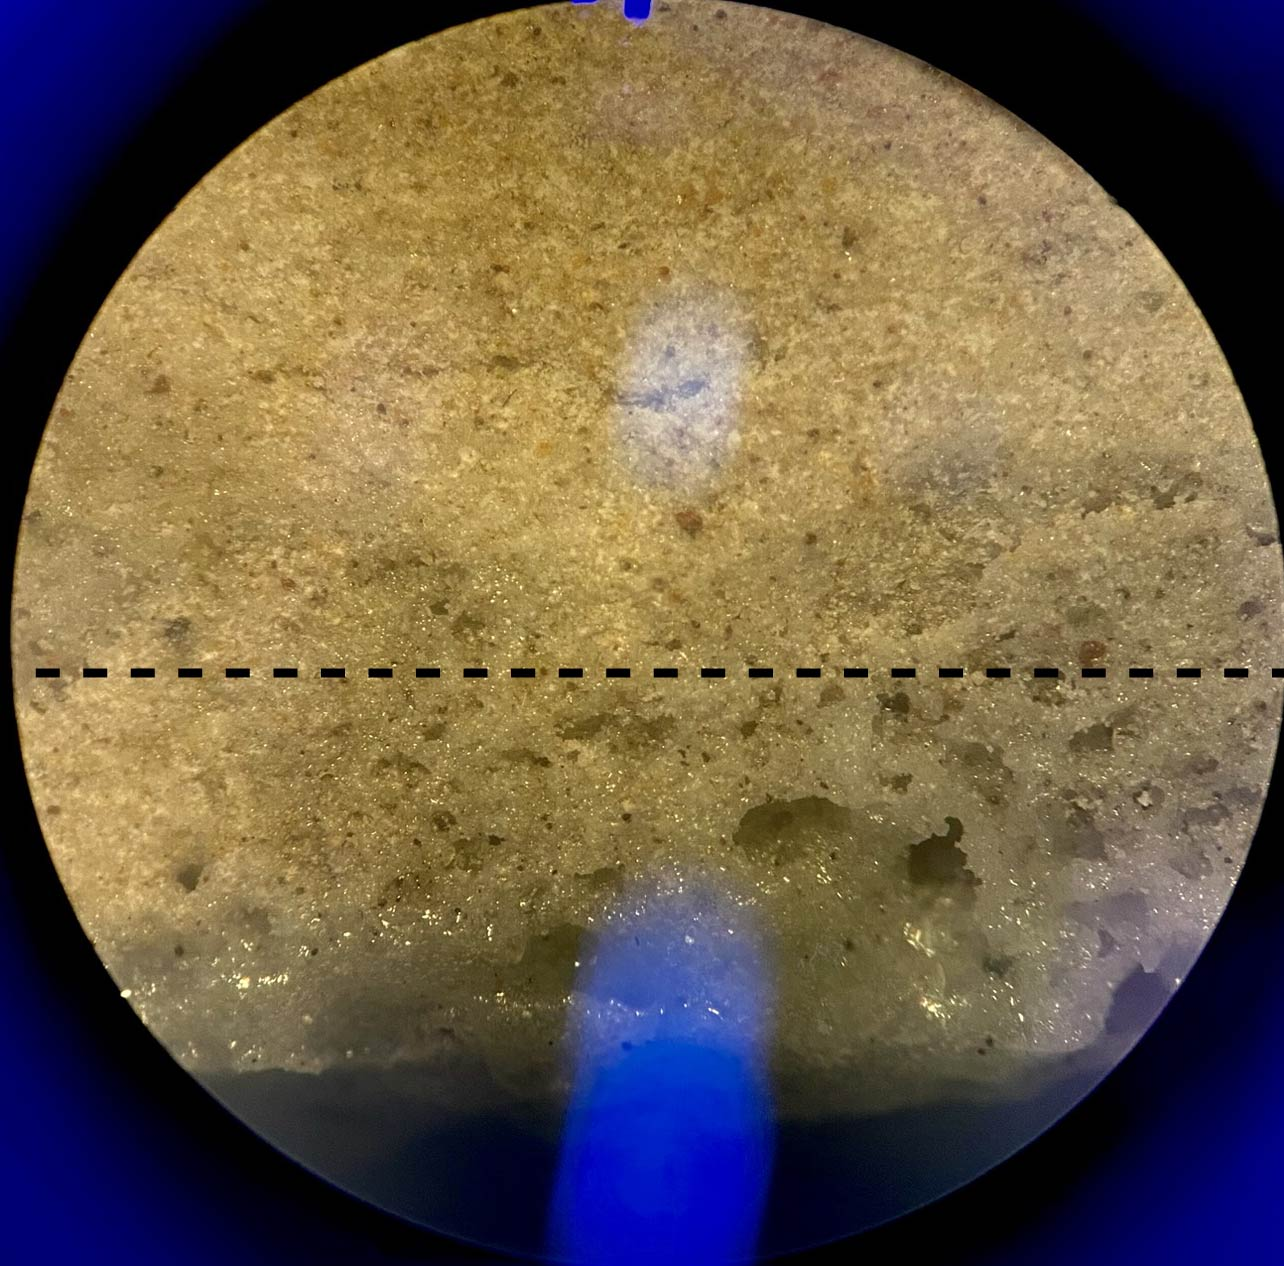
\includegraphics[width=0.5\linewidth]{Graphics/Densification.jpg}
    \caption{Vitrificacion de la membrana}
    \label{fig:vitrification}
\end{figure}

Durante el proceso de pulido, muchas fracturas de menor profundidad presentes en las membranas precursoras son eliminadas, sin embargo, otras de mayor profundidad se mantienen hasta las membranas finales como se muestra en la figura \ref{fig:pulido}. 

\begin{figure}
    \centering
    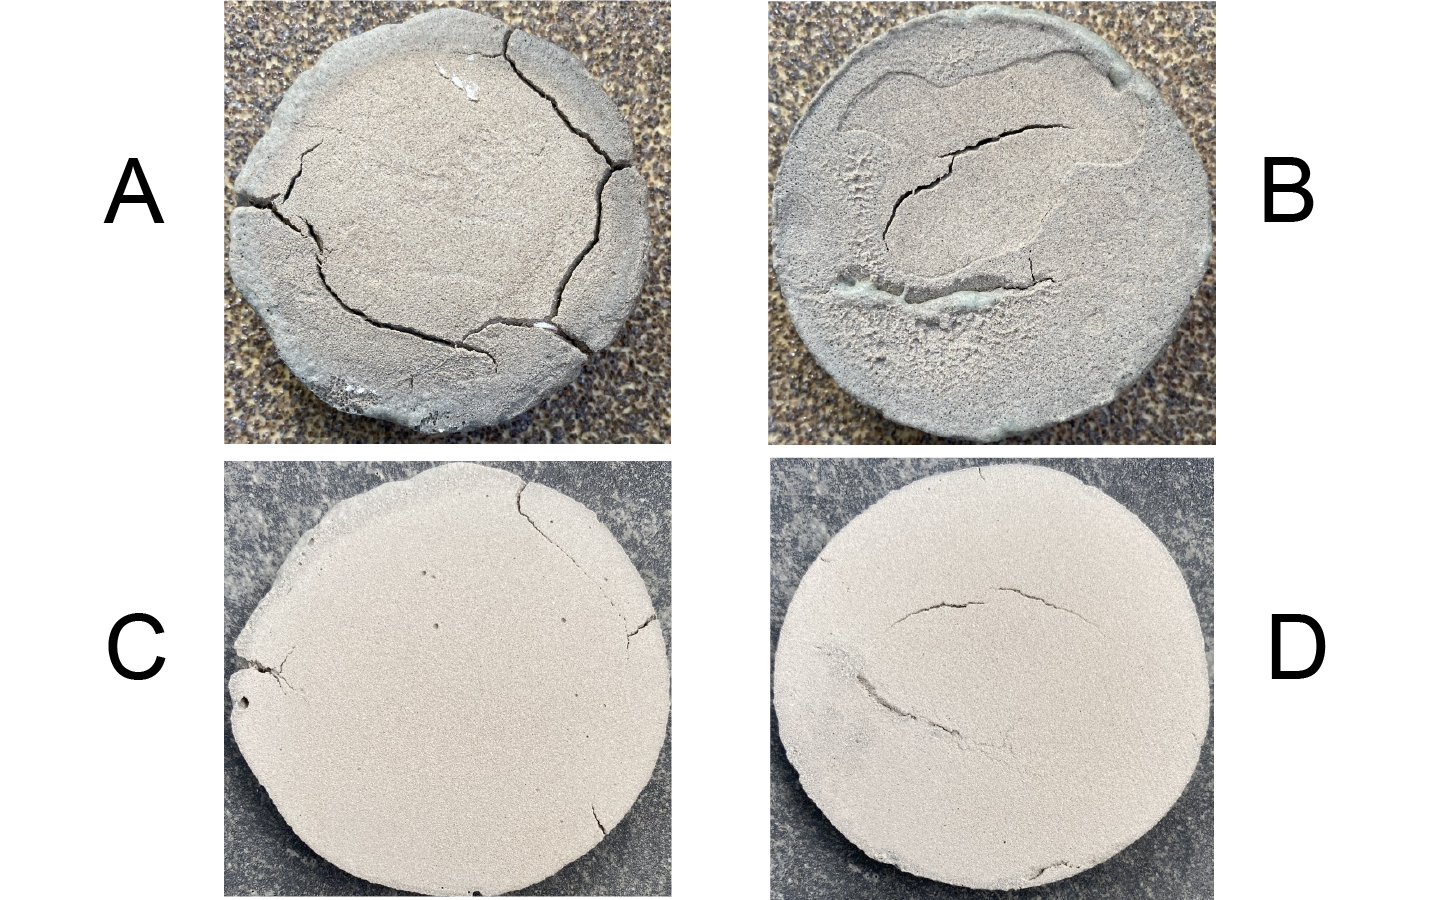
\includegraphics[width=0.5\linewidth]{Graphics/Membranes collage.png}
    \caption{pulido de las membranas. A y B representan las caras superiores e inferiores respectivamente previo al pulido, mienras que C  y D representan las caras superiores e inferiores respectivamente luego del proceso de pulido}
    \label{fig:pulido}
\end{figure}

\subsection{Estabilidad quimica de las membranas}

La Figura \ref{fig:EstabilidadQuimica} muestra la pérdida de peso en las membranas al ser sometidas a soluciones ácidas (HCl pH = 1) y básicas (NaOH, pH = 13). De forma general, a medida que la fracción de CBCA aumenta en la estructura de la membrana, en inmersión en soluciones ácidas hay un aumento en la actividad química, por lo que la introducción de CBCA en la composición de las membranas las hace más susceptibles al ataque ácido. Este comportamiento puede explicarse porque la CBCA contiene fases lábiles como carbonatos de calcio y sales alcalinas (K, Na), así como fracciones amorfas de sílice, que tienden a disolverse en medio fuertemente ácido, generando una mayor pérdida de masa.

Por otro lado, la tendencia es opuesta en soluciones alcalinas: a medida que las fracciones de CBCA aumentan en la composición de las membranas, la ganancia de peso o actividad química disminuye, por lo que existe menos deposición en las membranas con mayores fracciones de CBCA en su estructura. Esto podría estar asociado a la formación de capas superficiales de geles o hidróxidos de silicato que precipitan en las superficies ricas en pumita, mientras que en membranas con mayor contenido de CBCA el equilibrio entre disolución y reprecipitación es más limitado, reduciendo así la ganancia neta de masa.

En comparación con las membranas obtenidas por \textcite{Rawat2018} a partir de caolín y ceniza volante, las membranas conformadas a base de Pumicita/CBCA si poseen una fuerte actividad química en medios ácidos y baja en medios alcalinos. Por lo que, las membranas M1 y M2 son recomendadas para la microfiltración de soluciones ácidas y las de tipo M4 y M5 para la microfiltración de soluciones alcalinas. 

\begin{figure}[ht]
    \centering
    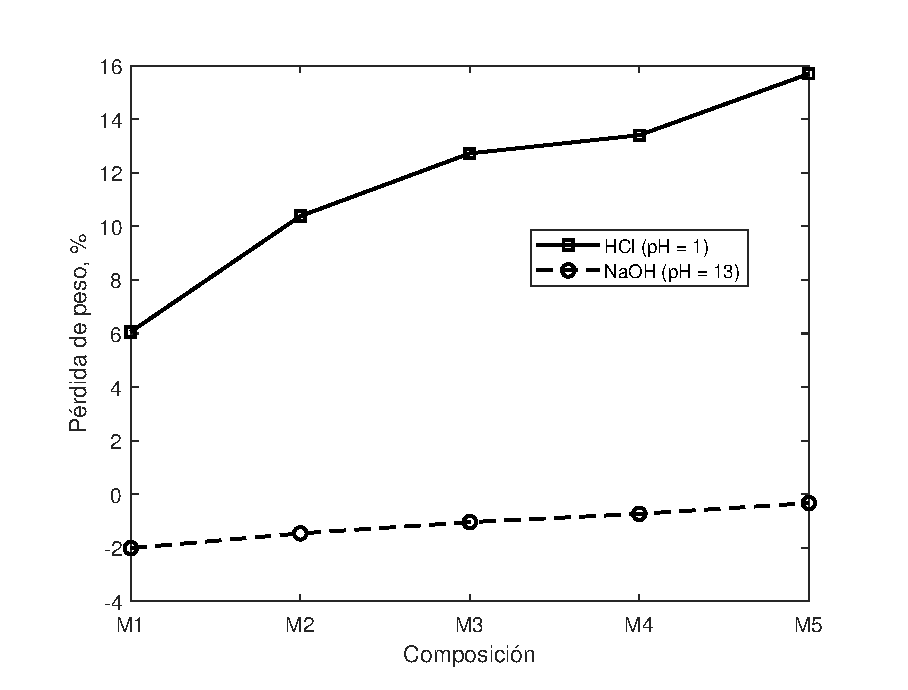
\includegraphics[width=0.5\linewidth]{Graphics/ChemStability.eps}
    \caption{Resultados de pruebas de estabilidad quimica}
    \label{fig:EstabilidadQuimica}
\end{figure}

\subsection{Efecto de la tasa de sinterizado y composición en el diámetro de poros y porosidad de la membrana. }

Para este análisis se utilizaron dos de los cinco tipos de membranas conformadas, M2 (75\% Pum 25\% CBCA) y M4 (25\% Pum 75\% CBCA) y se realizó un diseño factorial $2^2$.

En la figura 9 y 10 se muestran los gráficos de efectos principales y de interacción para la media de diámetro de poros. El gráfico de efectos principales muestra que tanto la composición de la membrana como la tasa de sinterizado tienen un efecto significativo en el diámetro de poros, disminuyendo para membranas con mayor fracción de CBCA y tasa de calentamiento. Esto es debido a que, por una parte la CBCA promueve la vitrificación en la estructura al momento de sinterizado, lo que podría implicar un bloqueo parcial de los poros, y por otra parte, el aumento en la tasa de calentamiento promueve los procesos de densificación, favoreciendo la coalescencia de partículas y la formación más rápida de cuellos. Como resultado, el diámetro de poro tiende a reducirse y la distribución de tamaños de poro se vuelve más estrecha, en concordancia con lo reportado por Chu et al. (1991). 

De acuerdo con el gráfico de interacción mostrado en la figura 10, el efecto de vitrificación en las membranas con mayor cantidad de CBCA (M4) se manifiesta de forma más pronunciada cuando el sinterizado es realizado con una tasa de calentamiento lenta, en comparación con el comportamiento observado cuando se utiliza una tasa de calentamiento alta, en la cual el efecto de la fracción de CBCA presente en las membranas no es significativo en el diámetro de poros, lo que sugiere que la cinética de densificación domina sobre los efectos que podrían aportar las composiciones variables de CBCA. 

Por su parte, los efectos principales y de interacción para la porosidad se muestran en las figuras 11 y 12. 
De acuerdo con los efectos principales mostrados en la figura 11, la fracción de CBCA en la membrana no presenta un efecto estadísticamente significativo. En contraste, la tasa de calentamiento si presenta un efecto significativo en la reducción de la porosidad de la membrana al aumentar la tasa de calentamiento de 4.75 a 6.82 °C/min, lo que evidencia que la cinética de densificación asociada a rampas de calentamiento más rápidas domina el comportamiento microestructural de las membranas. 

\begin{figure}
    \centering
    \includegraphics[width=0.7\linewidth]{Graphics/Grafico de efectos principales de Diametro de poros, μm.png}
    \includegraphics[width=0.7\linewidth]{Graphics/Grafico de interacciones Diametro de poros, μm.png}
    \caption{Grafico de Efectos Principales e Interacciones para Diámetro de poros}
    \label{fig:EfectosPrinDiametroPoros}
\end{figure}

\newpage
\section{CONTRIBUCIÓN DE AUTORÍA CRediT}

\section{DECLARACIÓN DE INTERESES CONTRAPUESTOS}

\section{DISPONIBILIDAD DE DATOS}

\section{AGRADECIMIENTOS}

\section{REFERENCIAS}

\printbibliography

\end{document}
